\newcommand{\communionTreeFig}{
%\begin{landscape}
\begin{figure*}[t]
{
    %\tiny
    %\scriptsize
    %\footnotesize
    %\small
    %\normalsize
    \begin{center}
    \begin{forest}
    %for tree={
    %    fit=band,% spaces the tree out a little to avoid collisions
    %    fit=tight,% spaces the tree out less
    %    fit=rectangle,
    %    inner sep=4,
    %}
    [{$g^{(s-e_1)(s-e_2)(s-e_3)(s-e_4)}$}
        [{$g^{(s-e_1)(s-e_2)}$}
            [{$g^{(s-e_1)}$}
                %[, no edge, tier=odd ]
            ]
            [{$g^{(s-e_2)}$}
                %[, no edge, tier=odd ]
            ]
        ]
        [{$g^{(s-e_3)(s-e_4)}$} 
            [{$g^{(s-e_3)}$}
                %[, no edge, tier=odd ]
            ]
            [{$g^{(s-e_4)}$}
                %[, no edge, tier=odd ]
            ]
        ]
    ]
    \end{forest}
    \end{center}
} % end of \tiny\scriptisize\whatever
\caption{A \communionTree (CT) over the set $\{e_1, e_2, e_3, e_4\}$.
The leaves store bilinear accumulators over the individual elements.
Every non-leaf node stores a bilinear accumulator over all elements from its subtree's leaves.}
\label{f:comm-tree}
\end{figure*}
%\end{landscape}
} % end of \newcommand

\newcommand{\accumulatedTreeFig}{
\begin{figure}[t]
    \centering
    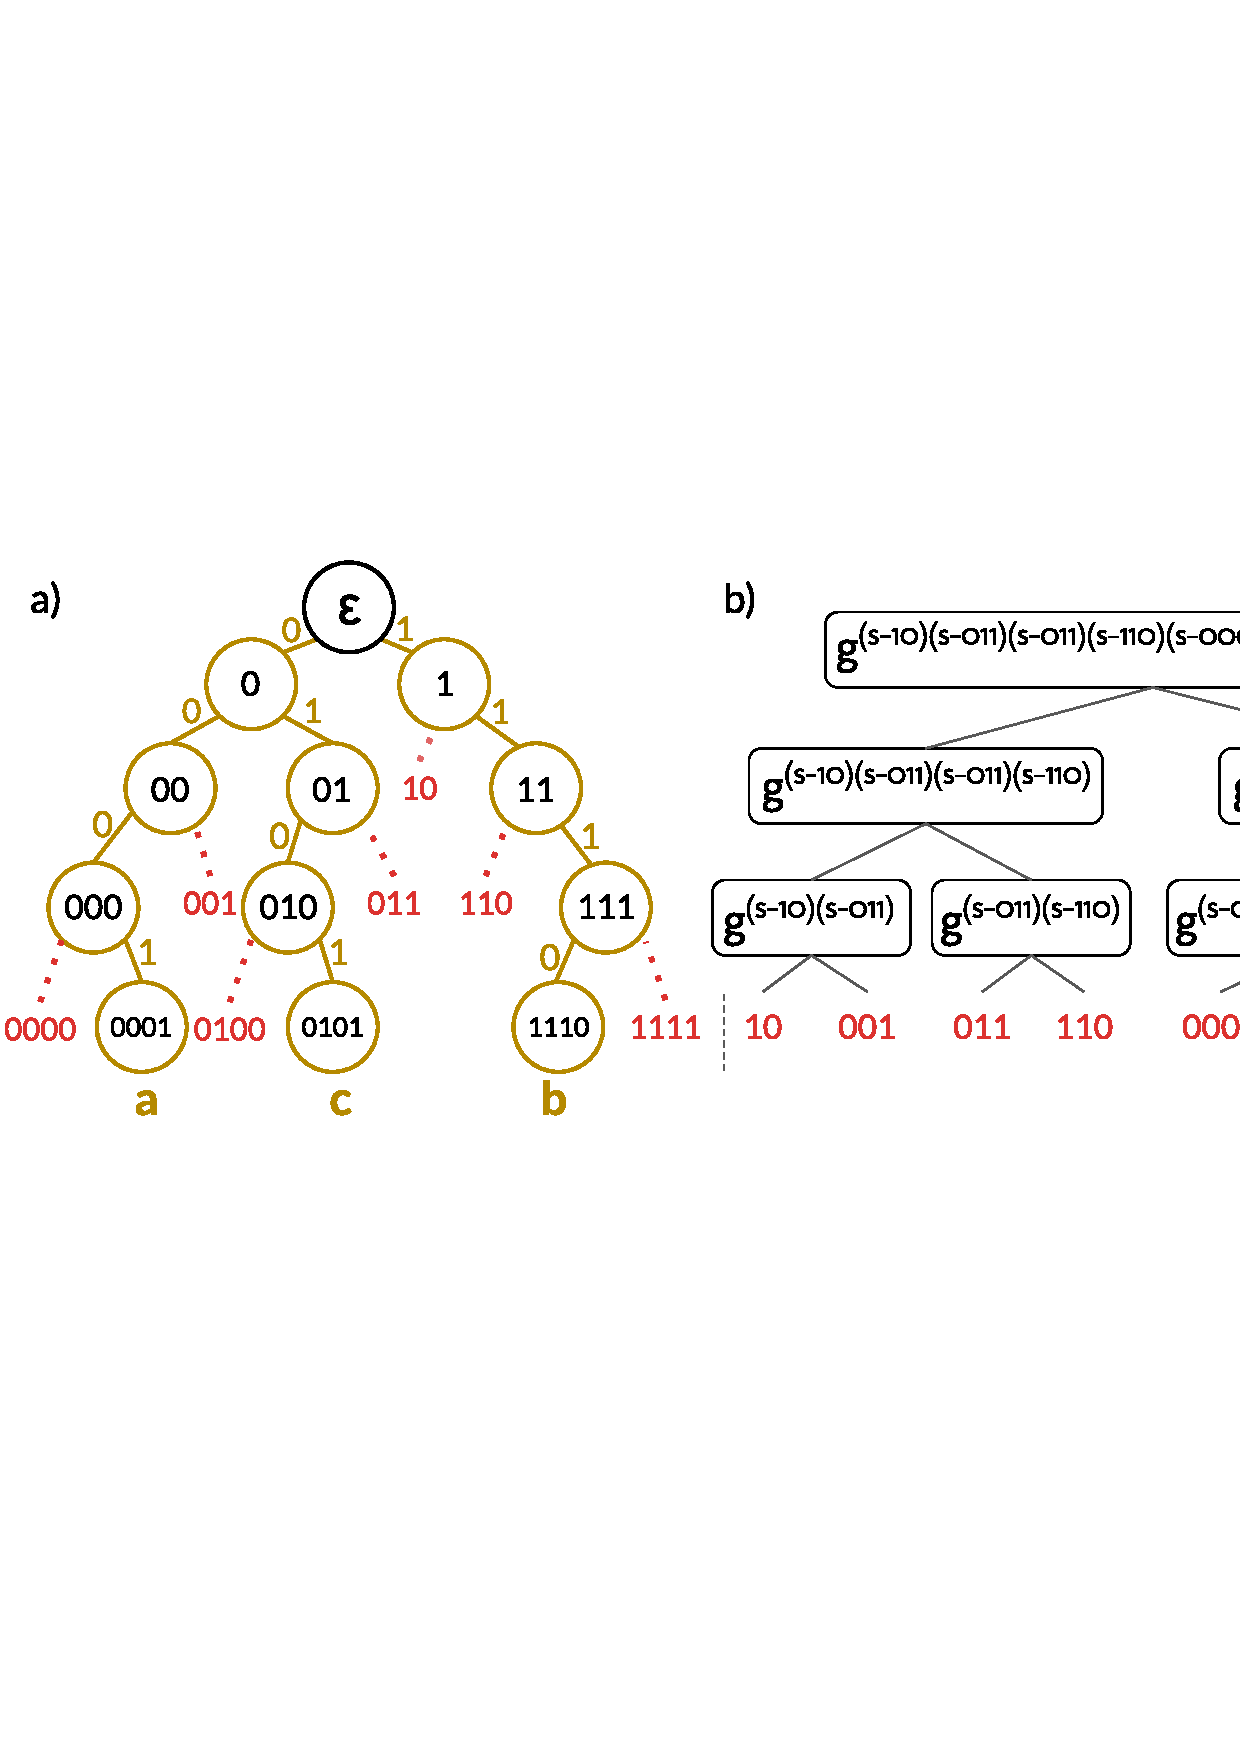
\includegraphics[width=.95\columnwidth]{figures-aad/AT.pdf}
    \vspace{-15em}
    \caption{
        On the left side, we depict a trie over set $S = \{a,b,c\}$.
        Each element is mapped to a unique path of length $4$ in the trie.
        (Here, $\lambda=2$.)
        Nodes that are not in the trie but are at its \textit{frontier} are depicted in \myred{\textbf{red}}.
        On the right side, we depict a \textit{\frontierCommunionTree} (FCT) corresponding to the set $S$.
        To prove that an element is not in $S$, we prove one of its prefixes is in the FCT.
        \label{f:accumulated-tree}}
    %\vspace{-2.5em}
\end{figure}
}

\newcommand{\forestFig}{
\begin{figure}[t]
    \centering
    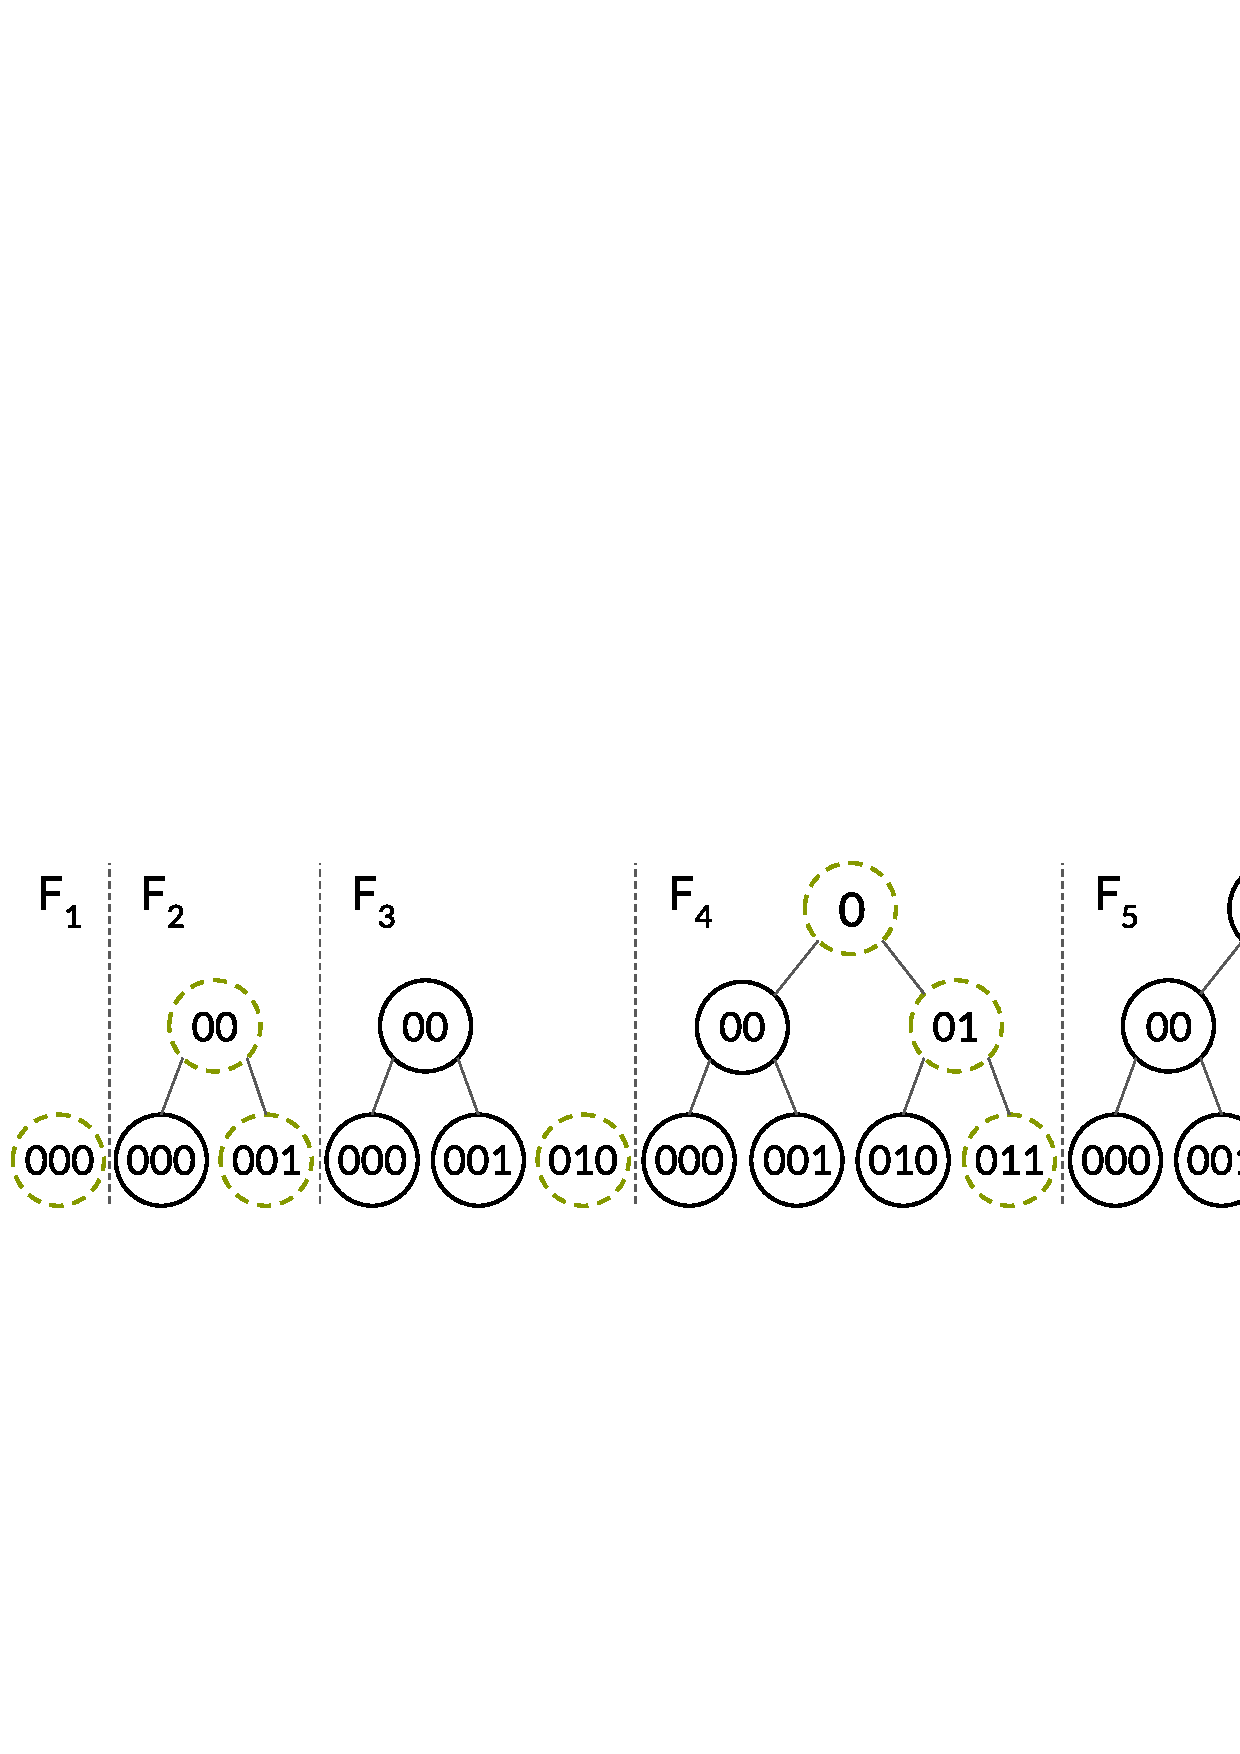
\includegraphics[width=.95\columnwidth]{figures-aad/forest.pdf}
    \vspace{-13em}
    \caption{
        A forest starting empty and going through a sequence of five appends.
        A forest only has trees of exact size $2^j$ for distinct $j$'s.
        A forest of $n$ leaves has \textit{at most} $\log{n}$ trees. 
    }
    \label{f:forest}
\end{figure}
}

\newcommand{\amortizedAasFig}{
\begin{figure}[t]
    \centering
    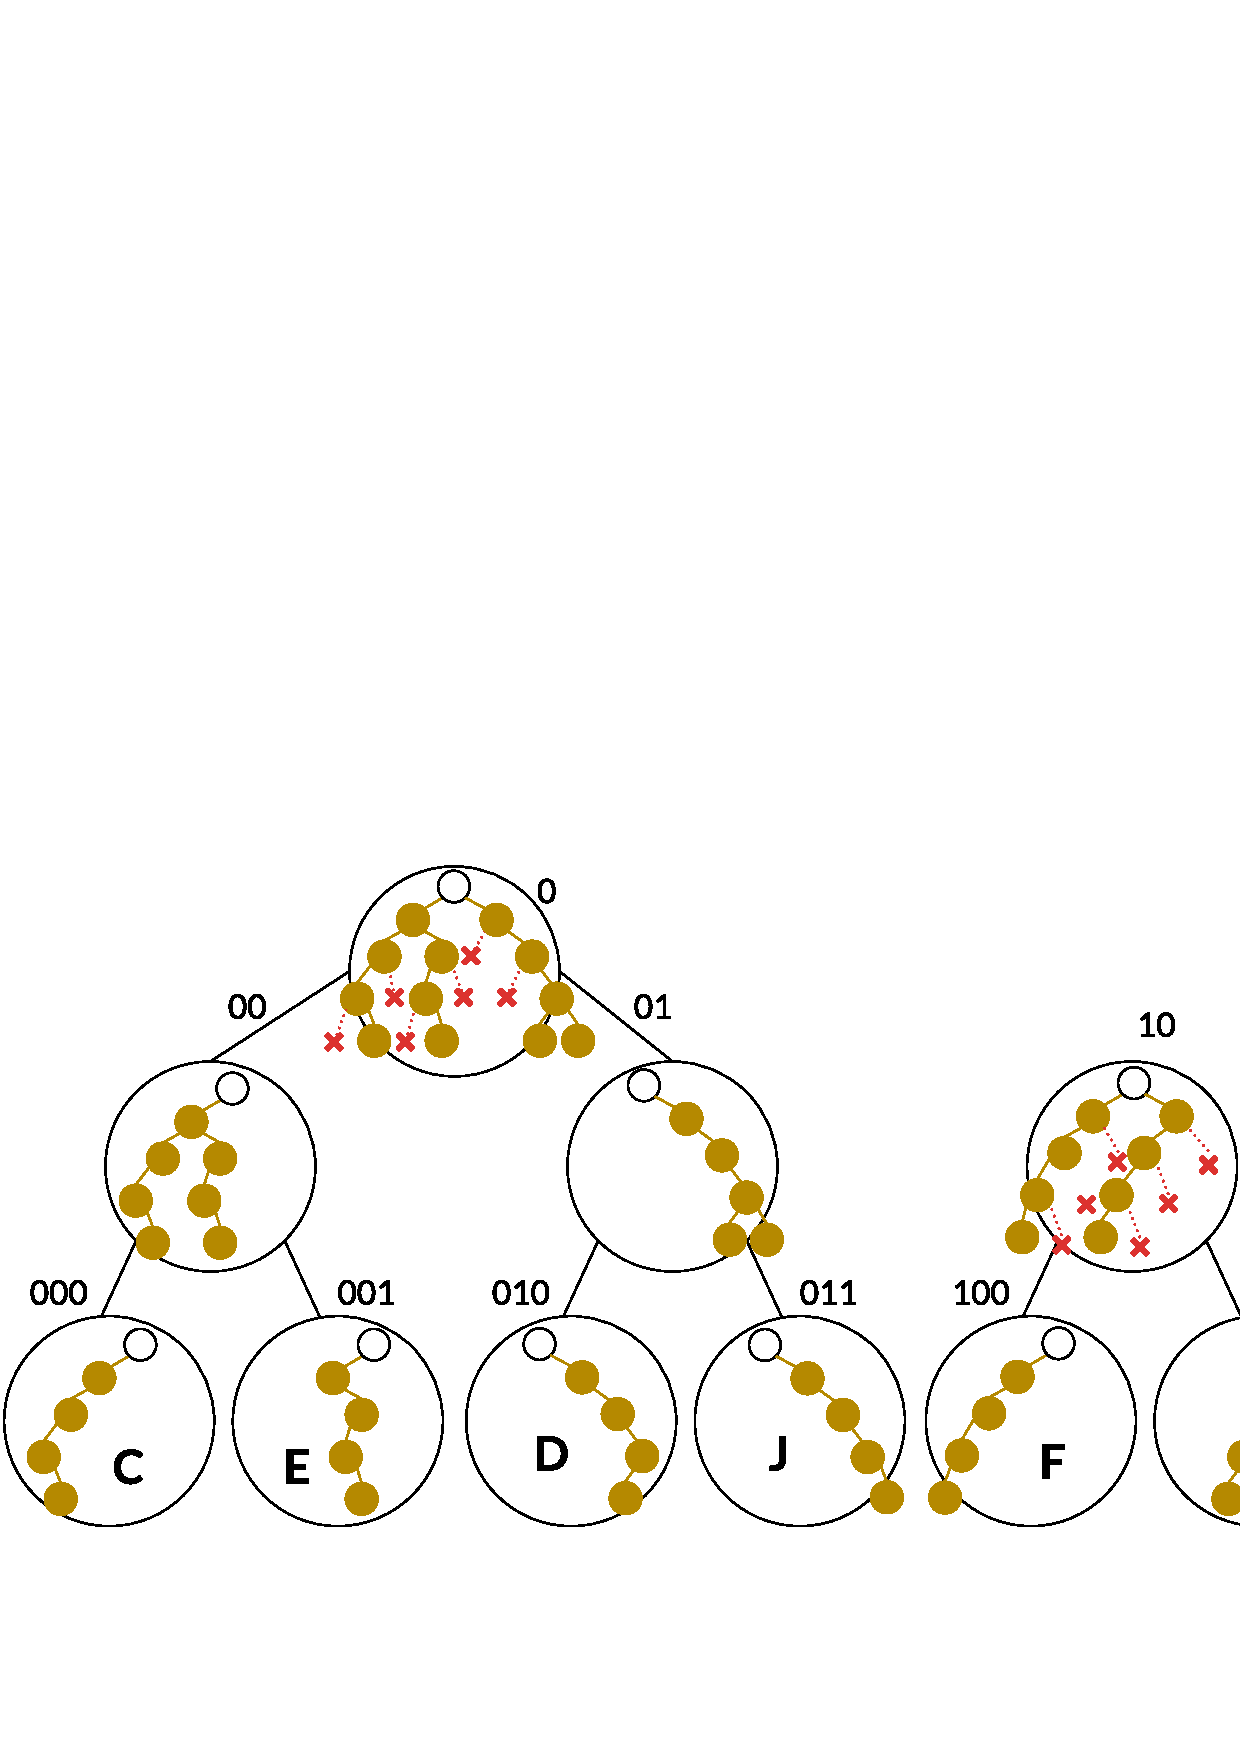
\includegraphics[width=.90\columnwidth]{figures-aad/accaas.pdf}
    \vspace{-1.7cm}
    \caption{
        A dynamic AAS with $\lambda=2$ for set $\{B,C,D,E,F,H,J\}$.
        Our AAS is a forest of PCTs with corresponding FCTs.
        Each node stores a prefix accumulator (and subset witness), depicted as a trie, in \myyellow{yellow}.
        Root nodes store an FCT, depicted as the missing \myred{red} nodes.
    }
    \label{f:accaas}
\end{figure}
}

This section presents our bilinear accumulator-based AAS construction.
We give a more formal, algorithmic description of this construction in \cref{s:aas:from-bilinear-acc:algorithms}.
We prove this construction secure under the $q$-SBDH and $q$-PKE assumptions in \cref{s:aas:from-bilinear-acc:proofs:membership-security}.
Finally, in \cref{s:aas:from-rsa-acc}, we present our RSA accumulator-based AAS.

As mentioned in \cref{s:intro:overview-techniques}, a bilinear accumulator over $n$ elements is already an AAS, but with two caveats: it is not fork-consistent (see \cref{def:aas:fork-consistency}) and it is computationally inefficient.
Specifically, proving (non)membership in a bilinear accumulator requires an $O(n)$ time polynomial division.
As a consequence, precomputing all $n$ membership proofs (naively) takes $O(n^2)$ time, which is prohibitive for most use cases.
Even worse, for non-membership, one must precompute proofs for all possible missing elements, of which there are exponentially many (in the security parameter $\lambda$).
Therefore, we need new techniques to achieve our desired polylogarithmic time complexity for computing both types of proofs in our AAS.

\subsection{Precomputing Membership with \communionTrees (CTs)}
\label{s:aas:from-bilinear-acc:ct}

\communionTreeFig

Our first technique is to deploy the bilinear accumulator in a tree structure, as follows.
We start with the elements $e_i$ as leaves of a binary tree (see \cref{f:comm-tree}).
Specifically, each leaf will store an accumulator over the singleton set $\{e_i\}$.
Every internal node in the tree will then store an accumulator over the union of the sets corresponding to its two children.
For example, the parent node of the two leaves corresponding to $\{e_i\}$ and $\{e_{i+1}\}$ stores the accumulator of the set $\{e_i,e_{i+1}\}$.
In this way, the root is the accumulator over the full set $S = \{e_1,\dots,e_n\}$ (see \cref{f:comm-tree}).

We stress that all accumulators in the tree use the same public parameters.
The time to compute all the accumulators in the tree is $T(n) = 2T(n/2) + O(n\log{n}) = O(n\log^2{n})$ where $O(n\log{n})$ is the time to multiply the characteristic polynomials of two sets of size $n$ in the tree.
We call the resulting structure a \textit{Comm(itment) Union Tree} or \emph{\communionTree} (CT) over set $S$, since every node in the tree is a commitment to the union of that node's childrens' committed sets.
A similar technique of ``unioning-and-then-accumulating'' sets in a tree first appeared in~\cite{CG10}.

A membership proof for element $e_i$ will leverage the fact that sets along the path from $e_i$'s leaf to the root of the \communionTree are subsets of each other.
The proof will consist of a sequence of \textit{subset witnesses} that validate this (computed as explained in \cref{s:prelim:bilinear-acc}).
Specifically, the proof contains the accumulators along the path from $e_i$'s leaf to the root, as well as the accumulators of all sibling nodes along this path (see \cref{f:comm-tree}).
The client verifies all these subset witnesses, starting from the singleton set $\{e_i\}$ in the leaf.
This convinces  him that $e_i$ is contained in the parent's accumulated set, which in turn is contained in its parent's accumulated set and so on, until the root.

Our CT approach gives us membership proofs of logarithmic size and thus logarithmic verification time.
Importantly, computing a \communionTree in $O(n\log^2{n})$ time implicitly computes all membership proofs ``for free''!
In contrast, building a standard billinear accumulator over $S$ would yield constant-size proofs but in $O(n^2)$ time for all $n$ proofs.
Unfortunately, CTs cannot (yet) precompute non-membership proofs, which we address next.

\accumulatedTreeFig

\subsection{Precomputing Non-membership by Accumulating Prefixes}
The \communionTree (CT) technique can efficiently precompute all $n$ membership proofs.
For non-membership though, we have to somehow precompute proofs for an exponential number of elements in the security parameter $\lambda$.
(Recall that an element is just a number $e\in \Fp$ where $p\approx 2^{2\lambda}$.)
For this, we build upon old ideas in computer science.

Specifically, we represent the set of elements as binary strings of length $2\lambda$ bits.
Thus, the set can be viewed as a \textit{trie} (see \cref{f:accumulated-tree}a).
As a consequence, when an element is not in the set, one of the prefixes of its binary string will not be in the trie.
Our key observation is that precomputing all proofs for such missing prefixes in effect precomputes all non-membership proofs.
This ``missing prefixes'' technique is also used in Micali et al.'s zero-knowledge sets~\cite{zks}.
We introduce it gradually below.

\subsubsection{\prefixCommunionTrees (PCTs)}
\label{s:aas:from-bilinear-acc:pct}
To efficiently precompute non-membership proofs, we slightly modify our CT construction into a \prefixCommunionTree (PCT).
As before, a parent's set is the union of its children's sets, but the key difference is that leaves will no longer store an individual element $e_i$ but will store all prefixes $\prefixes(e_i)$ of its binary representation.
We assume this representation is $2\lambda$ bits (or is made so using a CRHF) and can be mapped to an element in $\Fp$ (which is also of size $\approx 2\lambda$ bits) and thus can be accumulated.

For example, a leaf that previously stored element $e_1$ with binary representation $0001$, will now store the set $\prefixes(e_1) = \{\varepsilon,0,00,000,0001\}$ (i.e., all the prefixes of the binary representation of $e_1$, including the empty string $\varepsilon$).
Also, for any set $S = \{e_1,\dots,e_n\}$, we define its \emph{prefix set} as $\prefixes(S) = \prefixes(e_1) \cup \dots \cup \prefixes(e_n)$.
For example, let $S =\{a=0001,b=0101,c=1110\}$.
Then, the root of $S$'s \prefixCommunionTree will contain a \textit{prefix accumulator} over $\prefixes(S) = \prefixes(a) \cup \prefixes(b) \cup \prefixes(c) = \{\varepsilon,0,1,00,01,11,000,010,111,0001,0101,1110\}$.
We refer to accumulators in PCT nodes as prefix accumulators since they accumulate prefixes of elements, rather than elements themselves.

The time to build a PCT for $S$ is $O(\lambda n\log^2{n})$ since there are $O(\lambda n)$ prefixes across all leaves.
Note that membership proofs in a PCT are the same as in CTs, with a minor change.
The internal nodes of the tree still store accumulators over the union of their children.
However, the children now have common prefixes, which will only appear once in the parent.
For example, two children sets have the empty string $\varepsilon$ while their parent set only has $\varepsilon$ once (because of the union).
As a result, it is no longer the case that multiplying the characteristic polynomials of the children gives us the parent's polynomial.
Therefore, we can no longer rely on the siblings as subset witnesses: we have to explicitly compute subset witnesses for each child w.r.t. its parent.
We stress that this does not affect the asymptotic time complexity of computing the PCT.
As before, the client starts the proof verification from the leaf, which now stores a prefix set $\prefixes(e_i)$ rather than a singleton set $\{e_i\}$.

\subsubsection{\frontierCommunionTree (FCTs)}
\label{s:aas:from-bilinear-acc:fct}
But how does a PCT help with precomputing non-membership proofs for any element $e'\notin S$?
First, note that to prove $e'\notin S$ it suffices to show that \textit{any one prefix $\rho$ of $e'$ is not contained in $\prefixes(S)$}.
Second, note that there might exist other elements $e''$ who share $\rho$ as a prefix.
As a result, the non-membership proof for $e'$ could be ``reused'' as a non-membership proof for $e''$.

This is best illustrated in \cref{f:accumulated-tree}a using our previous example where $S =\{a,b,c\}$.
Consider elements $d= \underline{011}1$ and $f = \underline{011}0$ that are not in $S$.
To prove non-membership for either element, it suffices to prove the same statement: $\underline{011}\notin \prefixes(S)$.
Thus, if we can identify all such shared prefixes, we can use them to prove the non-membership of (exponentially) many elements.

First, note that prefix accumulator of a set $S$ is just a \textit{trie}, as depicted in \cref{f:accumulated-tree}a.
The key idea is to keep track of the prefixes at the ``frontier'' of the trie, depicted in \myred{\textbf{red}} in \cref{f:accumulated-tree}a.
Informally, these \textit{frontier prefixes} are prefixes that are \textit{not} in the trie but have a \textit{parent} in the trie (e.g., 011 is not in the trie but its parent 01 is).
We immediately notice that to prove non-membership of any element, it suffices to prove non-membership of one of these frontier prefixes!
In other words, elements that are not in $S$ will have one of these as a prefix.
We can formally define the \textit{frontier} of $S$ as:
\begin{align*}
    F(S) &= \{\rho \in \{0,1\}^{\le 2\lambda}: {\rho\not \in \prefixes(S)} \wedge {\parent(\rho) \in \prefixes(S)}\}\text{,}
\end{align*}
where $\parent(\rho)$ is $\rho$ without its last bit (e.g., $\parent(011) = 01$).
Note that the size of $F(S)$ is $O(\lambda n)$, proportionate to $\prefixes(S)$.

Most importantly, from the way $\prefixes(S)$ and $F(S)$ are defined, for any element $e'$, it holds that $e'\not\in S$ if, and only if, some prefix of $e'$ is in $F(S)$. 
Therefore, proving non-membership of $e'$ boils down to proving two statements: (i) some prefix of $e'$ belongs to $F(S)$, and (ii) $\prefixes(S) \cap F(S) = \varnothing$.
We stress that the latter is necessary as a malicious server may try to craft $F(S)$ in a false way (e.g., by adding some prefixes both in $\prefixes(S)$ and in $F(S)$).

To prove (i), we build a \communionTree over $F(S)$ which gives us precomputed membership proofs for all $\rho \in F(S)$ (see \cref{f:accumulated-tree}b).
We refer to this tree as the \emph{\frontierCommunionTree (FCT)} for set $S$, to the proofs as \textit{frontier proofs}, and to the accumulators in the tree as \textit{frontier accumulators}.
To prove (ii), we compute a \emph{disjointness witness} between sets $\prefixes(S)$ and $F(S)$, as described in \cref{s:prelim:polycommit} (i.e., between the root prefix accumulator and the root frontier accumulator).
The time to build a FCT for $S$ is $O(\lambda n\log^2{n})$ since $F(S)$ has $O(\lambda n)$ elements.
The disjointness witness can also be computed in $O(\lambda n\log^2{n})$ time.

\subsection{From Static to Dynamic AAS}

Combining all the above techniques, we obtain a \textit{static} AAS that does \textit{not yet} support updates efficiently (nor append-only proofs).
This construction consists of: (a) a PCT for $S$, (b) a FCT for $S$, and (c) a disjointness witness for $\prefixes(S)$ and $F(S)$ (i.e., between the root prefix and frontier accumulators).
The height of the PCT is $O(\log n)$ and the height of the FCT is $O(\log{(\lambda n)})$ so the size and verification time of a (non)membership proof is $O(\log{n})$.
The digest is just the root prefix accumulator of the PCT. 

\subsubsection{Appending Efficiently in Polylogarithmic Time}
Our AAS should \textit{efficiently} support appending new elements to $S$. 
The main challenge here is that updating the PCT and FCT as well as the disjointness witness after each update is very expensive (i.e., at least linear time in their size).
To address this we use a classic ``amortization'' trick from Overmars~\cite{overmars} also used in~\cite{distributed-acc}. 
Specifically, our AAS will consist not of one PCT for the entire set $S$, but of a \textit{forest} of PCTs and their corresponding FCTs.
The idea is to maintain a partitioning of $S$ with $1 + \floor{\log{|S|}}$ disjoint subsets, each of a distinct size $2^i$.

\forestFig

Initially, we start with no elements in the AAS.
When the first element $e_1$ is appended, we build its PCT over the set $\{e_1\}$, its FCT and a disjointness witness.
Together, these make up the \textit{CT-pair} of a set $S$ (in this case, $S=\{e_1\}$).
When the second element $e_2$ is appended, we ``merge'': we build a CT-pair over $\{e_1, e_2\}$.
We define the \textit{size of a CT pair} as the size of its set $S$ (in this case, the size is 2 since $S=\{e_1,e_2\}$).
The rule is we always merge equal-sized CT-pairs.
When $e_3$ is appended, we cannot merge it because there's no other CT-pair of size 1.
Instead, we create a CT-pair over $\{e_3\}$.

In general, after $2^\ell - 1$ appends, we end up with $\ell$ separate CT-pairs corresponding to sets of elements $S_1,\dots,S_\ell$.
The final set is $S=\bigcup_{j=1}^{\ell} S_j$ where $|S_j| = 2^j$.
The evolution of such a forest is depicted in \cref{f:forest} and the final data structure can be seen in \cref{f:accaas}.
In \cref{s:aas:from-bilinear-acc:asymptotics}, we show this approach gives us an $O(\lambda n\log^3 {n})$  \textit{amortized} append time.
Fortunately, generic \textit{de-amortization} techniques~\cite{overmars,overmars-van-leeuwen} can be used to obtain an $O(\lambda n\log^3 {n})$ \textit{worst-case} append time.

\amortizedAasFig

The downside of our amortized approach is that proving non-membership becomes slightly more expensive than in the static AAS data structure from above.
Specifically, now the server needs to prove non-membership in each CT-pair separately, requiring an $O(\log{n})$ frontier proof in each of the $O(\log{n})$ FCTs.
This increases the non-membership proof size to $O(\log^2 n)$.
On a good note, membership proofs remain unaffected: the server just sends a path to a leaf in \textit{one} of the PCTs where the element is found.
Finally, the AAS digest is set to the root prefix accumulators of all PCTs and has size $O(\log{n})$.
We analyze the complexity of our AAS in \cref{s:aas:from-bilinear-acc:asymptotics}.

\subsubsection{Logarithmic-sized Append-only Proofs}
Our append-only proofs are similar to the ones in history trees~\cite{ht}.
% Recall that when we merge the PCTs for $S_1, S_2$ and build a new PCT, (i) we compute its new root as the accumulator of $\prefixes(S_1) \cup \prefixes(S_2)$, (ii) we set the two old roots as the new root's children and (iii) we compute subset witnesses between the old roots and the new root.
% Thus, the old roots become children nodes in the new PCT.
% In fact, because every append to the AAS triggers a sequence of merges, we can generalize the above statement: after a sequence of appends, \textit{some} of the old roots in the old AAS will become descendants of a new root in the new AAS.
% The remaining old roots, if any, will remain as (new) roots in the new forest (e.g., root 0 from $F_4$ to $F_5$ in \cref{f:forest}).
% Our append-only proof leverages the above invariant.
An append-only proof must relate the root prefix accumulator(s) in the old AAS to the root prefix accumulator(s) in the new AAS.
We'll refer to these as ``old roots'' and ``new roots'', respectively.
Specifically, it must show that every old root either (i) became a new root or (ii) has a path to a new root with valid accumulator subset witnesses at every level.
Such a path is verified by checking the subset witnesses between every child and its parent, exactly as in a membership proof.
At the same time, note that there might be new roots that are neither old roots nor have paths to old roots (e.g., root 111 in $F_5$ from \cref{f:forest}).
The proof simply ignores such roots since they securely add new elements to the set.
To summarize, the append-only proof guarantees that each old root (1) has a valid subset path to a new root or (2) became a new root.

\paragraph{Ensuring Fork Consistency.}
For gossip protocols to work~\cite{CSP+15,DPV+18}, our AAS must be fork-consistent.
Interestingly, append-only proofs do not imply fork consistency.
For example, consider a server who computes an AAS for set $\{e_1\}$ and another one for the set $\{e_2\}$. 
The server gives the first set's digest to user $A$ and the second digest to user $B$.
Afterwards, he appends $e_2$ to the first set and $e_1$ to the second one, which ``joins'' the two sets into a common set $\{e_1,e_2\}$.
The append-only property was not violated (as the two users can deduce independently) but fork consistency has been: the two users had diverging views that were subsequently merged.

To avoid this, we will ``Merkle-ize'' each PCT using a CRHF $\Hb$ in the standard manner (i.e., a node hashes its prefix accumulator and its two children's hashes).
Our AAS digest is now set to the Merkle roots of all PCTs, which implicitly commit to all root prefix accumulators in the PCTs.
As a result, after merging PCTs for elements $e_1$ and $e_2$, the Merkle root of the merged PCT will differ based on how appends were ordered: $(e_1,e_2)$, or $(e_2,e_1)$.
Thus, violating fork consistency becomes as hard as finding a collision in $\Hb$.
(We prove this in \cref{s:aas:from-bilinear-acc:proofs:fork-consistency}.)

\subsection{Asymptotic Analysis}
\label{s:aas:from-bilinear-acc:asymptotics}

Suppose we have a \textit{worst-case} AAS with $n$ = $2^i - 1$ elements.

\paragraph{Append Time.}
First, let us analyze the time to merge two size-$n$ CT-pairs for two sets $S_1$ and $S_2$ into a size-$2n$ CT-pair for their union $S=S_1 \cup S_2$.
To compute $S$'s PCT, we need to (i) compute its prefix accumulator, (ii) set its children to the ``old'' prefix accumulators of $S_1$ and $S_2$ and (iii) compute subset witnesses for $S_1 \subset S$ and for $S_2\subset S$.
Since $|S_1|=|S_2|=n$, operations (i), (ii) and (iii) take $O(\lambda n \log^2{n})$ time.
Finally, we can compute $S$'s FCT from scratch in $O(\lambda n\log^2 n)$ time.

Now, consider the time $T(n)$ to create an AAS over a set $S$ with $n = 2^\ell$ elements (without loss of generality).
Then, $T(n)$ can be broken into:
\begin{itemize}
    \item The time to create a CT-pair over the children of $S$ of size $n/2$ (i.e., $2T(n/2)$).
    \item The time to merge these two CT-pairs, including computing subset witnesses (discussed above)
    \item The time to compute the FCT of $S$ (discussed above).
\end{itemize}
More formally, $T(n) = 2T(n/2) + O(\lambda n\log^2{n})$ which simplifies to $T(n) = O(\lambda n\log^3{n})$ time for $n$ appends.
Thus, the \textit{amortized} time for one append is $O(\lambda \log^3 {n})$ and can be de-amortized into \textit{worst-case} time using generic techniques~\cite{overmars,overmars-van-leeuwen}.

\paragraph{Space.}
The space is dominated by the FCTs, which take up $O(\lambda n/2) + O(\lambda n/4) + \dots + O(1) = O(\lambda n)$ space.
(When accounting just for the prefix accumulators, PCTs only take up $O(n)$ space.)

\paragraph{Digest Size.}
The digest is $O(\log{n})$-sized where $n$ is the size of the set.
We can make the digest constant-sized by hashing all Merkle roots together.
Then, we can include the Merkle roots as part of our append-only and lookup proofs, without increasing our asymptotic proof sizes.

\paragraph{Membership Proof Size.}
Suppose an element $e$ is in some PCT of the AAS .
To prove membership of $e$, we show a path from $e$'s leaf in the PCT to the PCT's root prefix accumulator consisting of constant-sized subset witnesses at every node.
Since the largest PCT in the forest has height $\log{(n/2)}$, the membership proof is $O(\log{n})$-sized.

\paragraph{Non-membership Proof Size.}
To prove non-membership of an element $e$, we show a frontier proof for a prefix of $e$ in every FCT in the forest.
The largest FCT has $O(\lambda n)$ nodes so frontier proofs are $O(\log{(\lambda n)})$-sized.
Because there are $O(\log{n})$ FCTs, all the frontier proofs are $O(\log{n}\log{(\lambda n)}) = O(\log^2{n})$-sized.

\paragraph{Append-only Proof Size.}
Our append-only proof is $O(\log{n})$-sized.
This is because, once we exclude common roots between the old and new digest, our proof consists of paths from each old root in the old forest up to a single new root in the new forest.
Because the old roots are roots of adjacent trees in the old forest, there will be a single $O(\log{n})$-sized Merkle path connecting the old roots to the new root.
In other words, our append-only proofs are similar to the append-only proofs from history trees~\cite{ht}.

\paragraph{Public Parameters.}
The server needs $q$-SDH public parameters, where $q = \Theta(\lambda n)$.
This is because, for an AAS of size $n$, it needs to build a trie of height $2\lambda$ over the $n$ keys.
In other words, the server has to accumulate $< (2\lambda+1) n$ prefixes which requires $((2\lambda +1) n)$-SDH parameters.
When verifying (non)membership proofs, a client must reconstruct a leaf prefix accumulator, which accumulates $2\lambda+1$ prefixes.
Thus, they only need $(2\lambda+1)$-SDH public parameters (see \cref{a:aas:setup}).
